% Shared standalone design for the editable figure reconstructions.
\documentclass[tikz,border=5pt,10pt]{standalone}
\usepackage[T1]{fontenc}
\usepackage[utf8]{inputenc}
\usepackage{newpxtext,newpxmath}
\usepackage[scaled=.94]{sourcesanspro}
\usepackage{pgfplots}
\pgfplotsset{compat=1.18}
\usetikzlibrary{arrows.meta,calc,positioning,decorations.pathreplacing,
  decorations.markings,patterns,matrix,shapes.geometric,fit,backgrounds,
  intersections,angles,quotes}
\definecolor{ink}{HTML}{203746}
\definecolor{accent}{HTML}{146C78}
\definecolor{muted}{HTML}{667780}
\definecolor{signalred}{HTML}{B94B44}
\color{ink}
\tikzset{>=Latex,line width=.8pt,
  every node/.style={font=\small},
  axis/.style={->,draw=muted,line width=.5pt},
  guide/.style={draw=muted,dashed,line width=.45pt},
  curve/.style={draw=accent,line width=1pt},
  marker/.style={circle,fill=accent,inner sep=1.5pt},
  labelbox/.style={fill=white,inner sep=2pt}}

\begin{document}
\begin{tikzpicture}
\begin{scope}
\node[font=\small\sffamily] at (2.1,3.4) {Capped inverse};
\draw[axis](0,0)--(4.6,0)node[right]{$\sigma$};\draw[axis](0,0)--(0,2.9)node[above]{$\mu_\tau(\sigma)$};
\draw[guide](1,0)node[below]{$\tau$}--(1,1.7);
\draw[guide](0,1.7)node[left]{$1/\tau$}--(1,1.7);
\draw[curve](0,1.7)--(1,1.7)plot[domain=1:4.3,samples=70](\x,{1.7/\x});
\draw[guide]plot[domain=.62:1,samples=30](\x,{1.7/\x});
\node at (2.1,-.85) {$\mu_\tau(\sigma)=\dfrac1{\max(\sigma,\tau)}$};
\end{scope}
\begin{scope}[shift={(6.5,0)}]
\node[font=\small\sffamily] at (2.1,3.4) {Tikhonov filter};
\draw[axis](0,0)--(4.6,0)node[right]{$\sigma$};\draw[axis](0,0)--(0,2.9)node[above]{$\mu_\lambda(\sigma)$};
\draw[curve]plot[domain=0:4.3,samples=90](\x,{1.7*\x/(1+\x*\x)});
\draw[guide](1,0)node[below]{$\sqrt\lambda$}--(1,.85)--(0,.85)node[left]{$\frac1{2\sqrt\lambda}$};
\fill[accent](1,.85)circle(1.5pt);
\draw[guide]plot[domain=.62:4.3,samples=80](\x,{1.7/\x});\node[muted,anchor=south west]at(1.45,1.18){$1/\sigma$};
\node at (2.1,-.85) {$\mu_\lambda(\sigma)=\dfrac{\sigma}{\sigma^2+\lambda}$};
\end{scope}
\node[muted]at(5.35,-1.65){Common axis scales; shown with $\tau=\sqrt\lambda>0$.};
\end{tikzpicture}
\end{document}
